\chapter{Chromatic numbers and chromatic polynomials}

\section{Computing chromatic numbers}

The vertex, edge, and total chromatic numbers can be computed using the \textit{SageMath} \cite{sagemath} function \verb|chromatic_number| and the appropriate conversions from Chapter~\ref{chap:clring_conversions}. Computing Tables~\ref{tab:platonic-chrom-nums} and~\ref{tab:archimedean-chrom-nums} took less than five seconds on a computer with the Apple M2 chip.

The following two tables provide an overview of vertex, edge, and total chromatic numbers, denoted by $\chi(G)$, $\chi'(G)$, and $\chi''(G)$ respectively, for the Platonic and Archimedean solids. Note that the edge chromatic number $\chi'(G)$ is also called the \textit{chromatic index}.

\begin{table}[H]
\centering
\begin{tabular}{l@{\hspace{1.5cm}}ccc}
\toprule
\textbf{Platonic} & \textbf{$\chi(G)$} & \textbf{$\chi'(G)$} & \textbf{$\chi''(G)$} \\
\midrule
tetrahedron & 4 & 3 & 5 \\
octahedron & 3 & 4 & 5 \\
cube & 2 & 3 & 4 \\
icosahedron & 4 & 5 & 6 \\
dodecahedron & 3 & 3 & 4 \\
\bottomrule
\end{tabular}
\caption{Vertex and edge chromatic numbers of Platonic graphs}
\label{tab:platonic-chrom-nums}
\end{table}

\begin{table}[H]
\centering
\begin{tabular}{l@{\hspace{1.5cm}}ccc}
\toprule
\textbf{Archimedean} & \textbf{$\chi(G)$} & \textbf{$\chi'(G)$} & \textbf{$\chi''(G)$} \\
\midrule
truncated tetrahedron & 3 & 3 & 4 \\
cuboctahedron & 3 & 4 & 5 \\
truncated cube & 3 & 3 & 4 \\
truncated octahedron & 2 & 3 & 4 \\
rhombicuboctahedron & 3 & 4 & 5 \\
snub cube & 3 & 5 & 6 \\
icosidodecahedron & 3 & 4 & 5 \\
truncated cuboctahedron & 2 & 3 & 4 \\
truncated icosahedron & 3 & 3 & 4 \\
truncated dodecahedron & 3 & 3 & 4 \\
rhombicosidodecahedron & 3 & 4 & 5 \\
snub dodecahedron & 4 & 5 & 6 \\
truncated icosidodecahedron & 2 & 3 & 4 \\
\bottomrule
\end{tabular}
\caption{Vertex and edge chromatic numbers of Archimedean graphs}
\label{tab:archimedean-chrom-nums}
\end{table}

Note that from the tables above, we see that indeed all the listed graphs have $\chi(G) \leq 4$. This is a consequence of the famous \textit{Four Color Theorem} \cite{appelhaken76} for planar graphs.

Using the result of \textit{Brooks' theorem} \cite{brooks41}, we know that the only graph among those listed for which $\chi(G) = \Delta(G) + 1$ should be the tetrahedron. This is indeed true, as can be verified by consulting Tables~\ref{tab:platonic-basic-props} and~\ref{tab:archimedean-basic-props}. 

By \textit{Vizing's theorem} \cite{misra92}, for every graph $G$ with maximum degree $\Delta(G)$, we have $\Delta(G) \leq \chi'(G) \leq \Delta(G) + 1$. This implies two classes of graphs. Class one contains graphs for which $\chi'(G) = \Delta(G)$, and class two contains those for which $\chi'(G) = \Delta(G) + 1$.

To determine which class the graphs of Platonic and Archimedean solids belong to, we compare the degrees at each vertex of the solids as shown in Tables~\ref{tab:platonic-basic-props} and~\ref{tab:archimedean-basic-props} with their chromatic indices in the tables above. We observe that all the solids are of Vizing class one. Note that this is not the case for all planar graphs. In fact, there exist planar graphs with $\Delta(G)$ from 2 up to 5 such that they are class two.

Similarly, for total coloring, Vizing's conjecture \cite{vizing68} states that for all graphs, we have $\Delta(G) + 1 \leq \chi''(G) \leq \Delta(G) + 2$. If the conjecture holds, then it again implies two classes of graphs. In the case of Platonic and Archimedean solids, it turns out that all of them except the tetrahedron belong to class with $\chi''(G) = \Delta(G) + 1$.

\section{Formula for computing chromatic polynomials}

The chromatic polynomial of any graph $G = (V, E)$ can be computed recursively using the following fact: When we fix two vertices $u$, $v$ such that $\{u,v\} \notin E$, we can split all colorings of $G$ into two disjoint groups. Let $d$ be the number of colorings of $G$ in which $u$ and $v$ are colored by different color and let $s$ be the number of colorings in which $u$ and $v$ are colored by same colors. Then the number of all colorings $P(G,x) = d + s$. Let $G+\{u,v\}$ be graph $G$ such that its set of edges is $E \cup \{u,v\}$. Let $G \cdot \{u,v\}$ be the graph $G + \{u,v\}$ where the edge $\{u,v\}$ is contracted into a single vertex. Then we can see that $d = P(G + \{u,v\},x)$ and $s = P(G \cdot \{u,v\},x)$. This fact yields the following formula \cite{chartrand2019}:
\begin{equation}\label{eqn:chrom_poly_nonedge}
 P(G,x) = P(G + \{u,v\},x) + P(G \cdot \{u,v\},x)
\end{equation}

The formula above serves as the recursive case of our computation, i.e., when the graph has some non-edge. In the other case—the base case—the graph has no non-edges and thus is a complete graph $K_n$ for some $n \in \mathbb{N}$. Then the chromatic polynomial is $P(K_n,x) = x \cdot (x-1) \cdot \ldots \cdot (x-n+1)$.

Consider this example: Given the graph of the tetrahedron $K_4$ and $X$, the family of proper vertex colorings, the chromatic polynomial is $P_{X}(K_4,x) = x \cdot (x-1) \cdot (x-2) \cdot (x-3)$. This can be seen if we label the vertices $v_1, v_2, v_3, v_4$ and imagine coloring them sequentially in the order of their labels. We have exactly $x$ colors available for the first vertex. For each subsequent vertex, we have one fewer color available to use.

\section{Chromatic polynomial of complete k-partite graphs with partition size 2}

In the following, let $\oplus$ denote the edge addition operation and let $\star$ denote the vertex identification operation. Let $G_{\oplus,\bar{e}}$ and $G_{\star,\bar{e}}$ describe the resulting graphs by applying the corresponding operation on some non-edge $\bar{e}$ of $G$. Let $\bar{E}$ denote the set of all non-edges of $G$.
\begin{defn}[set of non-edges]
    Let $G=(V,E)$ be a graph. We denote by $\bar{E} = \bar{E}(G) = \binom{V}{2} \setminus E$ the set of non-edges of $G$.
\end{defn}

\begin{defn}[vertex identification operation]
    For a graph $G=(V,E)$ and a non-edge $\{u,v\}$, we define the resulting graph $G_{\star,\{u,v\}} = (V',E')$ as follows:
    \begin{enumerate}
        \item $V' := (V \setminus \{u,v\}) \cup \{w\}$
        \item $E' = (\binom{V'}{2} \cap E) \cup \{\{w,x\} : \{u,x\} \in E \vee \{v,x\} \in E\}$
    \end{enumerate}
    In the above, we assume that $w \notin V$.
\end{defn}

Notice that for each $\bar{e} = \{u,v\} \in \bar{E}(G)$, we have $|\bar{E}(G_{\star,\bar{e}})| < |\bar{E}(G)|$. This is because $\{u,v\} \notin \bar{E}(G_{\star,\bar{e}})$, and also for the new vertex $w$, we have: 
\[
\{w,x\} \in \bar{E}(G_{\star,\bar{e}}) \implies \{u,x\} \in \bar{E}(G) \wedge \{v,x\} \in \bar{E}(G)
\]
In other words, the number of non-edges after the $\star$ operation always decreases.

\begin{lemma}
\label{lemma:non-edge_set_size}
    Let $G = K_{k \times (<n)}$ be a complete $k$-partite graph where each independent set has a size of at most $n$. Then, for any non-edge $\bar{e} \in \bar{E}(G)$ and $o \in \{\oplus,\star\}$, we have that: 
    \[
    |\bar{E}(G_{o,\bar{e}})| = |\bar{E}(G)| - 1
    \]
\end{lemma}

\begin{proof}
    Consider any $\bar{e} \in \bar{E}$. The operation $\oplus$ removes $\bar{e}$ from $\bar{E}$ and keeps the other non-edges intact, so the lemma holds for this case. For the case of the $\star$ operation, $\bar{E}(G_{\star,\bar{e}})$ will no longer contain the non-edge $\bar{e} = \{v,u\}$. Also, since the graph is complete $k$-partite, there exists no $w \in V(G) \setminus \{v,u\}$ such that $\{w,v\} \in \bar{E}$ or $\{w,u\} \in \bar{E}$. This means that after the $\star$ operation, all other non-edges will remain being non-edges. Also, the $\star$ operation does not create any new non-edges. This concludes the proof.
\end{proof}

\begin{lemma}
\label{lemma:indistinguishability}
    Let $G = K_{k \times (<n)}$ be a complete $k$-partite graph where each independent set has a size of at most $n$. Then, for any two non-edges $\bar{e}, \bar{f} \in \bar{E}(G)$ and $o \in \{\oplus,\star\}$, we have that:
    \[
    G_{o,\bar{e}} = G_{o,\bar{f}}
    \]
\end{lemma}

\begin{proof}
    Both $\bar{e}$ and $\bar{f}$ are non-edges between vertices from partitions of size $2$. Such partitions are all indistinguishable, so the resulting graph is the same in both cases $G_{o,\bar{e}}$ and $G_{o,\bar{f}}$.
\end{proof}

\begin{claim}
    Let $K_{k \times 2}$ be a complete $k$-partite graph where each independent set has size $2$. Then it holds that: 
    \begin{equation}\label{eqn:chromatic-pascal}
        P(K_{k \times 2},x) = \sum_{i=0}^{k} \binom{k}{i} P(K_{2k-i},x)
    \end{equation}
\end{claim}

\begin{proof}
    We base our proof on using the recursive algorithm for computing chromatic polynomials using the formula \ref{eqn:chrom_poly_nonedge} above. Let $G_{o_1,\ldots,o_n}$ be a graph resulting from applying the operations $o_1$ to $o_n$ in the corresponding order. By using Lemma \ref{lemma:indistinguishability} this graph is well defined, as the resulting graph is always the same irrespective of the particular choice of non-edges we apply the operations $o_1, \ldots,o_n$ to.

    In every step of the recursion, we divide the problem of calculating $P(G,x)$ into calculating the sum of $P(G_{\oplus,\bar{e}},x)$ and $P(G_{\star,\bar{e}},x)$. The recursion stops when there exists no non-edge $\bar{e} \in \bar{E}$ i.e. $G$ is a complete graph. By Lemma \ref{lemma:non-edge_set_size}, the recursion depth is equal to the number of non-edges of the original graph $K_{k\times 2}$ for every branch of the recursion. For $K_{k\times 2}$, this is equal to $k$. This means that each branch of the recursion ends with a graph $G_{o_1,\ldots,o_k}$ where $o_i \in \{\oplus,\star\}$. For a sequence of operations $s=o_1,\ldots,o_k$ let us denote $s_{\star} = |\{ i : o_i   =\star\}|$ i.e. the number of vertex identification operations performed throughout the sequence. Then we have $G_s = K_{2k-s_{\star}}$ because every $\star$ operation removes exactly one vertex from the original graph. Let $S$ be the set of all possible sequences of $k$ operations. Then for $G=K_{k\times 2}$, we have $P(G,x)= \sum_{s\in S}P(G_s,x)$. This follows from the fact that there is a one-to-one correspondence between branches of the recursion and sequences in $S$. We obtain the final formula by identifying all sequences with the same number of $\star$ operations, which produces the binomial coefficients in the final formula. 
\end{proof}


A particular example that demonstrates the claim above is the graph of the octahedron $K_{2,2,2} = K_{3 \times 2}$. According to formula \ref{eqn:chromatic-pascal}, we have \[ P(K_{3 \times 2},x) = P(K_6,x)+3P(K_5,x) + 3P(K_4,x)+P(K_3,x)\] as illustrated in the figure below.

\begin{figure}[H]
    \centering
    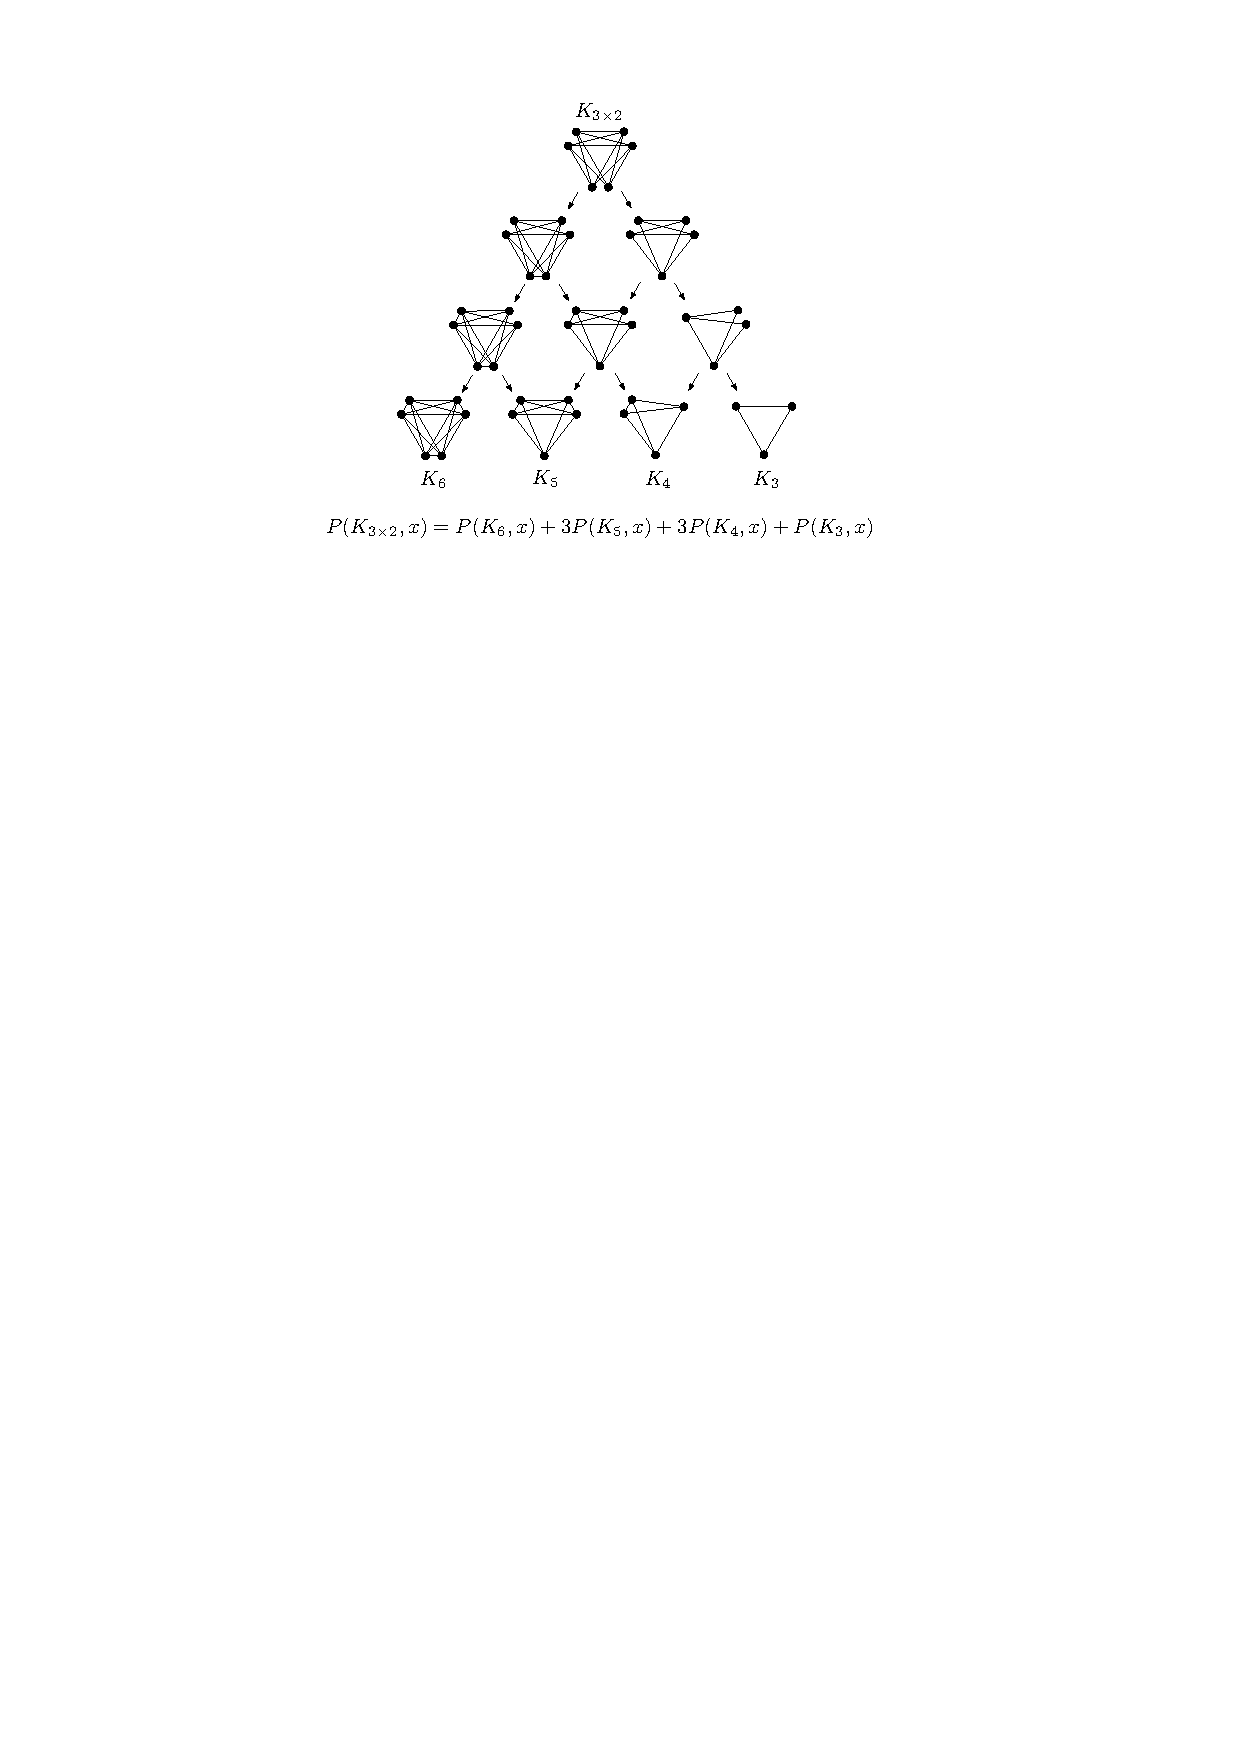
\includegraphics[width=0.8\textwidth]{Resources/Figs/octahedral_pascal_demo.pdf}
    \caption{Demonstration of formula \ref{eqn:chromatic-pascal} on a graph of the octahedron. Arrows pointing left correspond to edge additions. Arrows pointing right correspond to non-neighbor vertex identifications. Note that for some arrows, the reader must also imagine the graph being rotated after applying the corresponding operation.}
\end{figure}

\section{Computing chromatic polynomials of Platonic and Archimedean solids}\label{sec:comp-chrompolys}

Because the graphs of Platonic and Archimedean solids are all planar, it follows that they are also sparse. Thus, it is not practical to use the recursive formula \ref{eqn:chrom_poly_nonedge} which has complete graphs as the base case. We can instead simply reorganize the terms and use the following formula:

\begin{equation}\label{eqn:chrompoly-edge}
    P(G,x) = P(G - \{u,v\},x) - P(G \cdot \{u,v\},x)
\end{equation}

where $G - \{u,v\}$ is a graph with edge $\{u,v\}$ deleted and $G \cdot \{u,v\}$ a graph with edge $\{u,v\}$ contracted. 

Using the formula above, we can no longer use the complete graph as a base case. Instead, we use the fact that for a tree on $n$ vertices $T_n$, we have $P(T_n,x) = x \cdot (x-1)^{n-1}$. This can be imagined by choosing a root vertex $r$ and directing all edges in $T_n$ toward $r$. Now we can color the vertices sequentially s.t. we start with $r$ and then we color direct children of $r$ and so on. To color $r$, we can use all $x$ colors. For any other vertex $v \neq r$, only the \textit{unique} parent $p$ of $v$ is colored which means that there are $x-1$ free colors for $v$. 

Note that we assume that the graph $G$ with which we started is connected. This assumption comes naturally, as we are dealing only with graphs of 3-dimensional solids. We also assume that in the recursive step we always pick an edge that lies on a cycle. In this way, we will never create a disconnected graph. In practice, finding such an edge is done using DFS.

An algorithm that uses formula \ref{eqn:chrompoly-edge} and the above assumptions is implemented in the \textit{SageMath} \cite{sagemath} software under the name \verb|chromatic_polynomial|. The time complexity of this algorithm is exponential in $E(G)$, the number of edges of the graph $G$ on input. Using this algorithm, it is possible to calculate chromatic polynomials of Platonic and Archimedean graphs with at most $48$ edges in the order of minutes.

A more detailed description of how the algorithm is implemented can be found in a technical report by Read \cite{read1987chromatic}.

In the table below, we provide examples of the chromatic polynomials we computed.

\begin{table}[H]
\centering
\begin{tabular}{lp{0.7\linewidth}}
\toprule
\textbf{Solid} & \textbf{Chromatic polynomial} \\
\midrule
tetrahedron & $x^{4} - 6x^{3} + 11x^{2} - 6x$ \\
octahedron & $x^{6} - 12x^{5} + 58x^{4} - 137x^{3} + 154x^{2} - 64x$ \\
cube & $x^{8} - 12x^{7} + 66x^{6} - 214x^{5} + 441x^{4} - 572x^{3} + 423x^{2} - 133x$ \\
\bottomrule
\end{tabular}
\caption{Chromatic polynomial of selected solids.}
\label{tab:selected-chrom-polys}
\end{table}


We are also able to calculate these polynomials for other solids. Nevertheless, these polynomials have the property that the leading exponent is equal to the number of vertices of the graph. This results in long polynomials, which we provide in Section \ref{sec:more-chrompolys} of the appendix. On the other hand, we can also get a sense of the number of colorings of our graphs by evaluating the polynomials at certain points. We do this in the following section.

\section{Evaluating the chromatic polynomial}

Below, we provide tables with evaluations of the chromatic polynomial of all the Platonic solids and some of the Archimedean solids. The reason for not including all Archimedean solids is mentioned in Section \ref{sec:comp-chrompolys}.

\begin{table}[H]
\centering
\begin{tabular}{l@{\hspace{0.5cm}}ccccccc}
\toprule
\textbf{Platonic solid} & \textbf{2} & \textbf{3} & \textbf{4} & \textbf{5} & \textbf{6} & \textbf{7} & \textbf{8} \\
\midrule
tetrahedron & $0$ & $0$ & $24$ & $120$ & $360$ & $840$ & $1\,680$ \\
octahedron & $0$ & $6$ & $96$ & $780$ & $4\,080$ & $15\,330$ & $45\,696$ \\
cube & $2$ & $114$ & $2\,652$ & $29\,660$ & $198\,030$ & $932\,862$ & $3\,440\,024$ \\
icosahedron & $0$ & $0$ & $240$ & $80\,400$ & $4\,012\,560$ & $\approx 10^{7}$ & $\approx 10^{8}$ \\
dodecahedron & $0$ & $7\,200$ & $\approx 10^{8}$ & $\approx 10^{11}$ & $\approx 10^{13}$ & $\approx 10^{14}$ & $\approx 10^{16}$ \\
\bottomrule
\end{tabular}
\caption{Evaluated chromatic polynomial of Platonic solids at points 2 to 8.}
\label{tab:platonic-chrompolys-evals}
\end{table}

\begin{table}[H]
\centering
\begin{tabular}{l@{\hspace{0.5cm}}cccccc}
\toprule
\textbf{Archimedean solid} & \textbf{2} & \textbf{3} & \textbf{4} & \textbf{5} & \textbf{6} & \textbf{7} \\
\midrule
truncated tetrahedron & $0$ & $120$ & $60\,000$ & $3\,410\,880$ & $\approx 10^{7}$ & $\approx 10^{8}$ \\
cuboctahedron & $0$ & $24$ & $9\,216$ & $772\,680$ & $\approx 10^{7}$ & $\approx 10^{8}$ \\
truncated cube & $0$ & $13\,440$ & $\approx 10^{9}$ & $\approx 10^{13}$ & $\approx 10^{15}$ & $\approx 10^{17}$ \\
truncated octahedron & $2$ & $378\,978$ & $\approx 10^{10}$ & $\approx 10^{13}$ & $\approx 10^{15}$ & $\approx 10^{17}$ \\
\bottomrule
\end{tabular}
\caption{Evaluated chromatic polynomial of Archimedean solids at points 2 to 7.}
\label{tab:archimedean-chrompolys-evals}
\end{table}

It is important to note that in Table \ref{tab:platonic-polys-evals} above, in column $n$, the entry does not correspond to the number of colorings with exactly $n$ colors but with \textbf{at most} $n$ colors. This means that colorings that used only a proper subset of the $n$ available colors are counted as well. Sometimes, we would like to avoid counting these colorings. For this reason, we show a method to arrive at the number of colorings using \textbf{exactly} n colors, in the section below.

\section{Number of colorings using exactly n colors}
\label{sec:num-clrings-exactly-n-clrs}

\begin{defn}[number of exact n-colorings]
    Let $P^*(G,n)$ be defined as the number of colorings of a graph $G$ using \textbf{exactly} $n$ colors.
\end{defn}

The number $P^*(G,n)$ can be calculated using a recursive formula, with the base case $P^*(G,\chi(G))=P(G,\chi(G))$. We introduce the formula in the following claim.

\begin{claim}\label{clm:exactly-n-colors}
    Let $G$ be a graph, and $n$ be a positive integer. Then:
    \begin{equation}\label{eqn:exactly-n-colors}
    P^*(G,n) = P(G,n) - \sum_{i=\chi(G)}^{n-1}\binom{n}{i}P^*(G,i)    
    \end{equation}
\end{claim}

\begin{proof}
    For the base case, where $n\le \chi(G)$, we have straightforwardly $P^*(G,\chi(G))=P(G,\chi(G))$, since there exist no colorings that use less than $\chi(G)$ colors.
    
    For the recursive case, let $n>\chi(G)$ be the number for which we want to calculate $P^*(G,n)$. We proceed by taking the value $P(G,n)$ and noticing that this value also calculates colorings using $n-1$, $n-2$, \ldots, $\chi(G)$ colors that we want to exclude. For $i \in \{\chi(G),\ldots,n-1\}$, how many colorings using $i$ colors have we calculated? A naive approach would be to simply subtract the value $P^*(G,i)$. The problem with this approach is that when we are allowed to use $n$ colors and have to use exactly $i$ of them, we can choose the set of $i$ colors to use in $\binom{n}{i}$ ways. Note that indeed all of the $\binom{n}{i}$ colorings use at most $n$ colors and are pairwise different. Using this observation, we can see that the correct value to subtract is $\binom{n}{i}P^*(G,i)$ for each $i$.
\end{proof}

Now, with formula \ref{eqn:exactly-n-colors} above in hand, we can use results from tables \ref{tab:platonic-chrompolys-evals} and \ref{tab:archimedean-chrompolys-evals} to compute the numbers of colorings using \textbf{exactly} n colors. See tables below:

\begin{table}[H]
\centering
\begin{tabular}{l@{\hspace{0.5cm}}ccccccc}
\toprule
\textbf{Platonic solid} & \textbf{2} & \textbf{3} & \textbf{4} & \textbf{5} & \textbf{6} & \textbf{7} & \textbf{8} \\
\midrule
tetrahedron & $0$ & $0$ & $24$ & $0$ & $0$ & $0$ & $0$ \\
octahedron & $0$ & $6$ & $72$ & $360$ & $720$ & $0$ & $0$ \\
cube & $2$ & $108$ & $2\,208$ & $17\,520$ & $57\,600$ & $80\,640$ & $40\,320$ \\
icosahedron & $0$ & $0$ & $240$ & $79\,200$ & $3\,533\,760$ & $\approx 10^{7}$ & $\approx 10^{8}$ \\
dodecahedron & $0$ & $7\,200$ & $\approx 10^{8}$ & $\approx 10^{11}$ & $\approx 10^{13}$ & $\approx 10^{14}$ & $\approx 10^{16}$ \\
\bottomrule
\end{tabular}
\caption{Number of colorings of Platonic solids using \textbf{exactly} n colors for n from 2 up to 8.}
\label{tab:platonic-chrompolys-exacts}
\end{table}

\begin{table}[H]
\centering
\begin{tabular}{l@{\hspace{0.5cm}}cccccc}
\toprule
\textbf{Archimedean solid} & \textbf{2} & \textbf{3} & \textbf{4} & \textbf{5} & \textbf{6} & \textbf{7} \\
\midrule
truncated tetrahedron & $0$ & $120$ & $59\,520$ & $3\,112\,080$ & $\approx 10^{7}$ & $\approx 10^{8}$ \\
cuboctahedron & $0$ & $24$ & $9\,120$ & $726\,840$ & $\approx 10^{7}$ & $\approx 10^{8}$ \\
truncated cube & $0$ & $13\,440$ & $\approx 10^{9}$ & $\approx 10^{13}$ & $\approx 10^{15}$ & $\approx 10^{17}$ \\
truncated octahedron & $2$ & $378\,972$ & $\approx 10^{10}$ & $\approx 10^{13}$ & $\approx 10^{15}$ & $\approx 10^{17}$ \\
\bottomrule
\end{tabular}
\caption{Number of colorings of Archimedean solids using \textbf{exactly} n colors for n from 2 up to 7.}
\label{tab:archimedean-chrompolys-exacts}
\end{table}

\section{Limitations of the chromatic polynomial}

The results we obtained above using the chromatic polynomial have two important limitations that arise because of the way the difference of two colorings is defined.

\subsection{Counting up to symmetries}

Firstly, it may happen that we consider two colorings as different even though they are just different rotations or reflections of each other. See examples of such colorings below:

\begin{figure}[H]
    \centering
    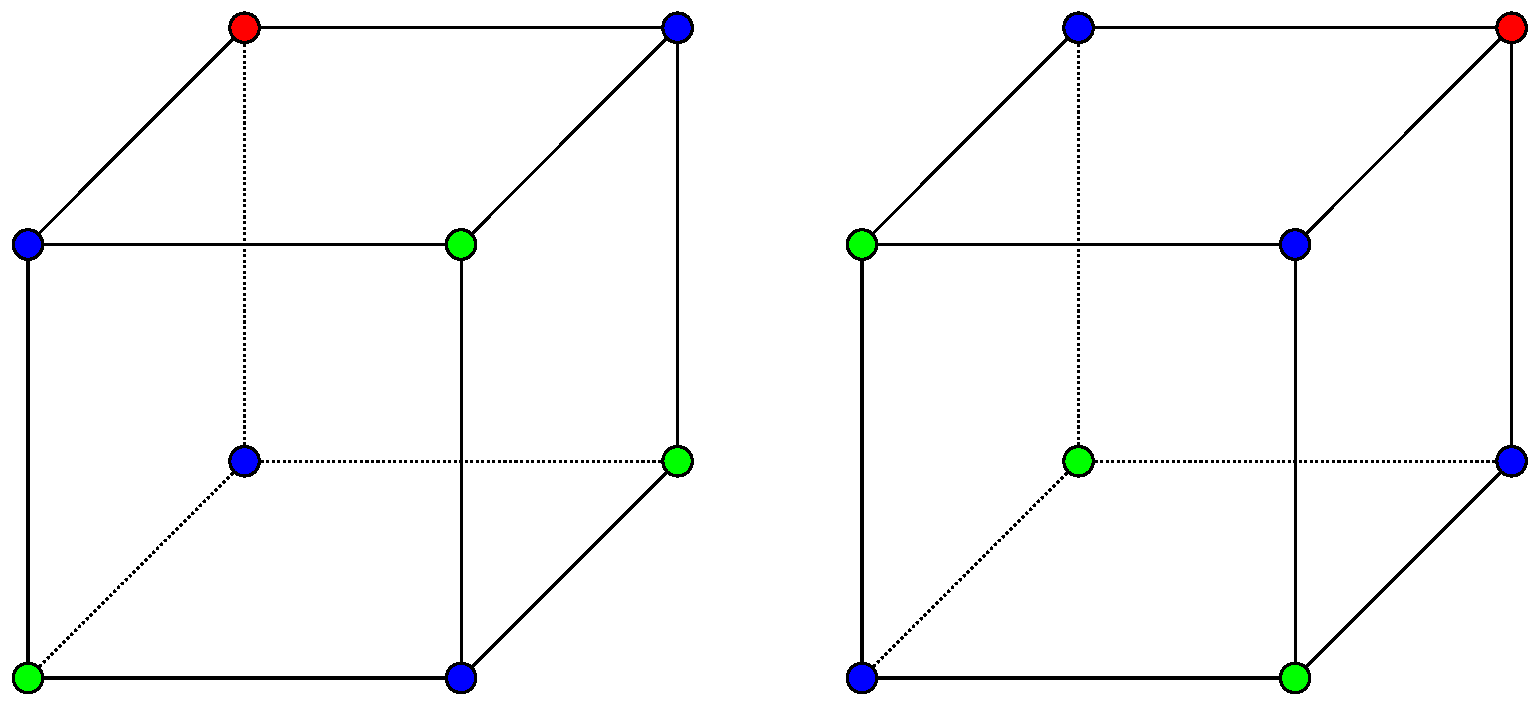
\includegraphics[width=0.75\textwidth]{Resources/Figs/cube_rotations_problem.pdf}
    \caption{Two 3-colorings of cube that are same up to symmetries}
    \label{fig:cube-clrings-same-up-to-symmetries}
\end{figure}

If we are interested only in colorings different up to symmetries, we need to use a method that is described in chapter \ref{chap:clrings-up-to-symmetries}.

\subsection{Counting up to labels of independent sets}

The second limitation arises when we need to view the colorings as partitions into independent sets irrespective of the particular names, or values, of the colors. Then, there can be cases of partitions which we count multiple times, because there exist different non-equal ways to label the colors. In other words, an independent set that is given the color red will be considered as different from the same independent set when it is given the color blue. See an illustration of this problem below:

\begin{figure}[H]
    \centering
    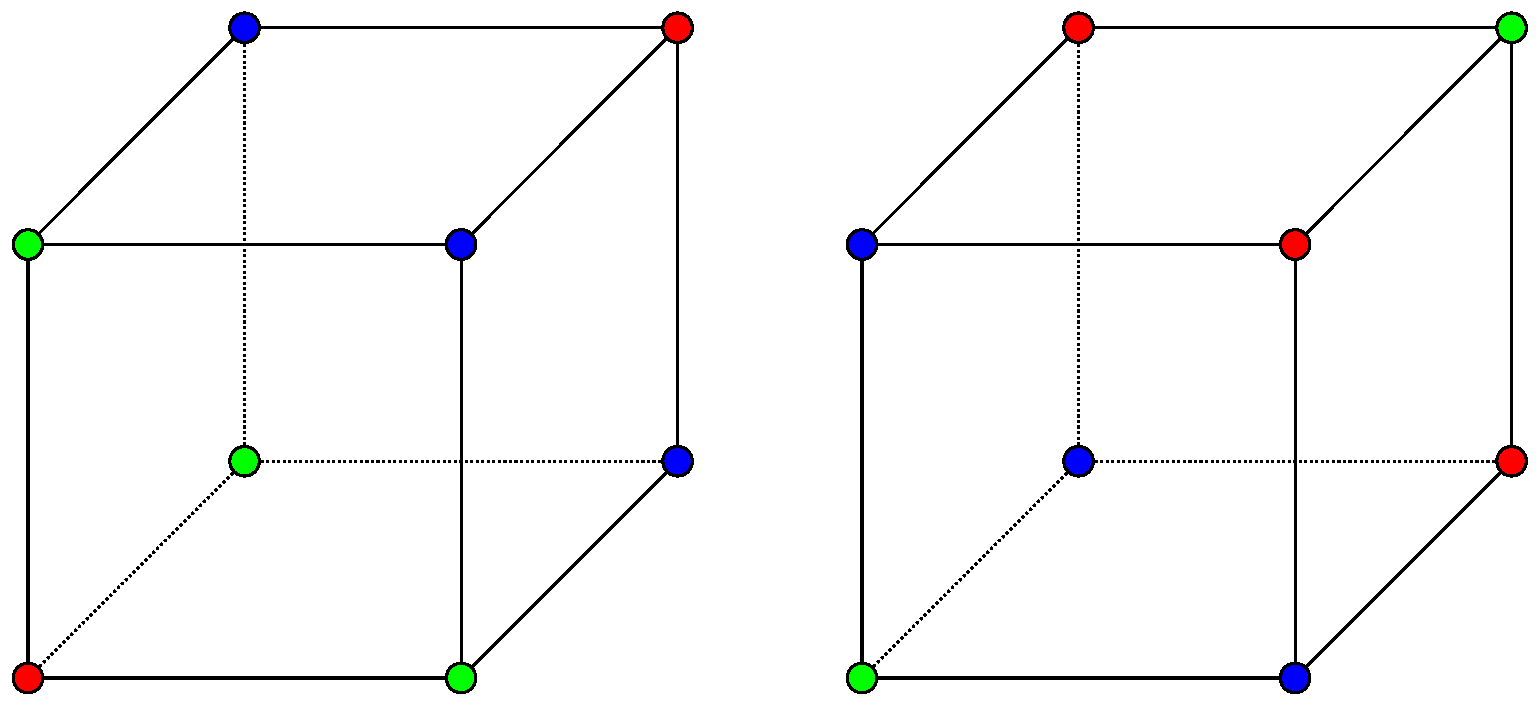
\includegraphics[width=0.75\textwidth]{Resources/Figs/cube_relabelings_problem.pdf}
    \caption{Two 3-colorings of cube that correspond to the same partition into independent sets}
    \label{fig:cube-clrings-same-partition}
\end{figure}

The problem of counting independent sets multiple times can be solved using the method described in Chapter \ref{chap:num-partitions-into-indep-sets}. 

Also, note that the two colorings in Figure \ref{fig:cube-clrings-same-partition} above are different up to symmetries, so the problems mentioned above are indeed different and must be handled separately.

